%             Exemple d'utilisation de la classe thesul
%             ------------------------------------------
%
%
% (de manière generale, les commandes de thesul sont celles
% qui ne sont pas complètement en minuscules)
%
% Voir la documentation complète pour plus de détails.
%
%
% D. Roegel, 30 mars 2013
%
\documentclass[10pt]{TUL/thesul}
%----------------------------------------------------------------------
%                     Chargement de quelques packages
%----------------------------------------------------------------------

% Si l'on veut produire une version PDF avec des hyperliens :
% \usepackage[pageanchor=false]{TUL/tulhypref}
\usepackage[hidelinks, pdftex]{TUL/tulhypref}

% Si on veut le style de bibliographie named :
%\usepackage{named}

% Pour les figures :
\usepackage{graphicx}

% Si on veut des mini-tables des matières (utiliser minitoc-hyper 
% en conjonction avec tulhypref) :
\usepackage[french]{minitoc}

\usepackage[backgroundcolor=blue!20!white, linecolor=black]{todonotes}
% \usepackage[disable]{todonotes}
\usepackage{titlesec}
\usepackage{url}
\usepackage[backend=biber, language=french, maxnames=5, citestyle=alphabetic,bibstyle=alphabetic,backref,abbreviate=false,dateabbrev=false,isbn=false,url=false,doi=true]{biblatex}

\addbibresource{these.bib}

% Structure
\newtheorem{theo}{Théorème}
\newtheorem{defi}{Définition}
\newtheorem{prop}{Proposition}
% \theoremstyle{remark}\newtheorem*{preuve}{Preuve}

% Abbreviations :
\newcommand{\xq}{x86}
\newcommand{\xs}{x86$\_$64}

\titleformat{\chapter}[display]
  {\bfseries\huge}
  {\filleft\Large\chaptertitlename~\thechapter}
  {3ex}
  {\titlerule\vspace{1.5ex}\filright}
  [\vspace{1ex}\titlerule]

%-------------------------------------------------------------------
%                             Marges
%-------------------------------------------------------------------

% pour positionner les vraies marges:
%\SetRealMargins{1mm}{1mm}

%-------------------------------------------------------------------
%                             En-têtes
%-------------------------------------------------------------------

% Les en-têtes: quelques exemples
%\UppercaseHeadings 
%\UnderlineHeadings
%\newcommand\bfheadings[1]{{\bf #1}}
%\FormatHeadingsWith{\bfheadings}
%\FormatHeadingsWith{\uppercase}
%\FormatHeadingsWith{\underline}
\newcommand\upun[1]{\uppercase{\underline{\underline{#1}}}}
\FormatHeadingsWith\upun

\newcommand\itheadings[1]{\textit{#1}}
\FormatHeadingsWith{\itheadings}

% pour avoir un trait sous l'en-tete:
\setlength{\HeadRuleWidth}{0.4pt}

%-------------------------------------------------------------------
%                         Les références
%-------------------------------------------------------------------

\NoChapterNumberInRef
\NoChapterPrefix

%-------------------------------------------------------------------
%                           Brouillons
%-------------------------------------------------------------------

% ceci ajoute une marque « brouillon » et la date
%\ThesisDraft

%-------------------------------------------------------------------
%                   Pour collecter un glossaire et un index
%-------------------------------------------------------------------

\makeglossary
\makeindex

\begin{document}





\OddHead={{\leftmark\rightmark}{\hfil\slshape\rightmark}}
\EvenHead={{\leftmark}{{\slshape\leftmark}\hfil}}
\OddFoot={\hfil\thepage}
\EvenFoot={\thepage\hfil}
\pagestyle{ThesisHeadingsII}

%-------------------------------------------------------------------
%                          Encadrements
%-------------------------------------------------------------------

% encadre les chapitres dans la table des matières:
% (ces commandes doivent figurer apres \begin{document}

\FrameChaptersInToc  
%\FramePartsInToc


%-------------------------------------------------------------------
%            Réinitialisation de la numérotation des chapitres
%-------------------------------------------------------------------

% Si la commande suivante est présente,
% elle doit figurer APRÈS \begin{document}
% et avant la première commande \part
% \ResetChaptersAtParts 

%-------------------------------------------------------------------
%               mini-tables des matières par chapitre
%-------------------------------------------------------------------

% préparer les mini-tables des matières par chapitre.
% (commande de minitoc.sty)
\dominitoc

%-------------------------------------------------------------------
%                         Page de titre:
%-------------------------------------------------------------------

\ThesisTitle{Analyse morphologique de logiciels malveillants auto-modifiants}
\ThesisDate{dd/mm/aaaa}
\ThesisAuthor{Aurélien Thierry}

% Type de la these
\ThesisUL

% Jury:

% (ne pas mettre de \\ apres la dernière entree)

% Exemple de création d'une nouvelle catégorie dans le jury:

\NewJuryCategory{family}{\it Membre de la famille :}
                        {\it Membres de la famille :}

\family={Mon frère\\Ma sœur}

\def\blanc{\hspace*{1cm}}

\President    = {Le président}
\Rapporteurs  = {Le rapporteur 1&de Paris\\
                 Le rapporteur 2\\
                 \blanc suite&taratata\\
                 Le rapporteur 3}
\Examinateurs = {L'examinateur 1&d'ici\\
                 L'examinateur 2}
%\Invites=       {}

% Création de la page de titre:
\MakeThesisTitlePage

% on peut en faire plusieurs:
%\MakeThesisTitlePage

%-------------------------------------------------------------------


%-------------------------------------------------------------------
%                          remerciements
%-------------------------------------------------------------------

%\DontFrameThisInToc
\begin{ThesisAcknowledgments}
Merci.
\end{ThesisAcknowledgments}

%-------------------------------------------------------------------
%                            dédicace
%-------------------------------------------------------------------

% \begin{ThesisDedication}
% Ah.
% \end{ThesisDedication}


%-------------------------------------------------------------------
%                  écriture de `Chapitre' et `Partie' 
%                      dans la table des matières
%-------------------------------------------------------------------

\WritePartLabelInToc
\WriteChapterLabelInToc

%-------------------------------------------------------------------
%                        table des matières
%-------------------------------------------------------------------

\tableofcontents

%-------------------------------------------------------------------
%              Exemple d'utilisation de \SpecialSection
%-------------------------------------------------------------------

% \SpecialSection{Introduction générale}


% Pour ne pas avoir le mot « Chapitre » au début de chaque chapitre.
% \NoChapterHead

\DontWriteThisInToc   
\listoffigures


% La commande \mainmatter permet de passer
% à la numérotation arabe (ce que fait \pagenumbering{arabic}) 
% et de faire commencer la nouvelle page 1 sur une page impaire.
% On évitera donc d'utiliser directement \pagenumbering{arabic}.
\mainmatter

\DontFrameThisInToc
\NumberThisInToc
\chapter{Introduction}
Ceci est une introduction.
\todo{Mettre une intro}

% \WriteThisInToc
% \FrameThisInToc
% \NumberThisInToc
\part{Désassemblage et analyse de binaires}

% \NumberThisInToc
\DontFrameThisInToc
\chapter{Assembleur}
% \newcommand{\xqq}{x862}

\todo[inline]{source -> ASM -> binaire // asm -> (désas) -> (décomp)}
Nous nous intéressons en premier lieu aux programmes malveillants fonctionnant sur des ordinateurs personnels.
Les programmes s'exécutant sur ces machines sont compilés afin d'être exécutés nativement dans le langage assembleur spécifique au processeur de la machine.

\section{Compilation et fichiers exécutables}
Un exécutable est en général d'abord écrit dans un langage de haut niveau. Chacun de ses modules est ensuite compilé en un fichier objet (binaire) encodant le langage assembleur spécifique à la machine. La dernière étape est l'édition de liens qui consiste à regrouper tous les fichiers objets en un exécutable unique.

Prenons l'exemple d'un simple \helloworld\ en C (Figure \ref{fig:helloword_c}). Il est uniquement composé d'un appel à la fonction \texttt{printf} permettant l'affichage, à l'exécution, de la chaîne de caractère ``Hello, world.''.
Une implémentation possible en assembleur \nasm\ \xq\ pouvant tourner sous une distribution GNU/Linux est donnée en figure \ref{fig:helloword_asm}. Il est alors composé de deux appels système vers le noyau Linux : une première (sys$\_$write) permettant l'affichage de la chaîne et une seconde (sys$\_$exit) permettant de fermer le processus.
On peut déjà remarquer que le programme est séparé en une section de données (.data) contenant la chaîne de caractère à afficher et une section de code (.text) contenant le code assembleur à exécuter.
\begin{figure}
\begin{lstlisting}[language={C}]
int main(int argc, char* argv[]){
  printf("Hello, world.");
}
\end{lstlisting}
\caption{Code C de \helloworld}
\label{fig:helloword_c}
\end{figure}


\begin{figure}
\begin{lstlisting}[language={[x86masm]Assembler}, escapechar=~]
section .data
msg     db      "Hello, world", 0xa	; ~La chaîne à afficher~
len     equ     $ - msg                 ; ~La taille de la chaîne~

section .text
global _start

_start:
; ~Afficher la chaîne de caractères~
mov     eax, 4      ; ~Numéro d'appel système (sys$\_$write)~
mov     ebx, 1      ; ~Premier argument : le fichier de sortie (ici stdout)~
mov     ecx, msg    ; ~Second argument : un pointeur vers la châine à afficher~
mov	edx, len    ; ~Troisième argument : la taille de la chaîne~
int     0x80        ; ~Appel effectif au noyau~

; ~Fermer proprement le programme~
mov     eax, 1      ; ~Numéro d'appel système (sys$\_$exit)~
mov	ebx, 0	    ; ~Premier argument : le code de retour (0 : normal)~
int     0x80	    ; ~Appel au noyau~
\end{lstlisting}
\caption{Code assembleur \xq\ de \helloworld}
\label{fig:helloword_asm}
\end{figure}

Le fichier binaire exécutable résultant de la compilation est un exécutable binaire pour Linux, sous format ELF.
% Le format ELF est structuré de la manière suivante. 
Comme indiqué sur la figure \ref{fig:structure_elf}, il contient des entêtes dans lesquels sont indiqués des informations générales sur le binaire telle que le point d'entrée du programme, les différentes sections du programme (leur taille, leurs adresses) et les différentes sections : ici une section .data (Figure \ref{fig:data_helloworld}) contient les données du programmes (dont la chaîne de caractères ``Hello World'') et une section .text (Figure \ref{fig:text_helloworld}) contenant le code assembleur à exécuter.
À l'instar de la figure \ref{fig:structure_elf} donnant une structure simplifiée du format ELF pour Linux, la figure \ref{fig:structure_pe} donne un aperçu du format des fichiers exécutables pour un binaire \xq\ sous Windows.

\begin{figure}
\begin{center}
\subfigure[Fichier ELF]{
\begin{tabular}[b]{|c|}
\hline
Entête ELF\\
\hline
Table des entêtes du programme\\
\hline
Section .text\\
\hline
Section .rodata\\
\hline
Section ...\\
\hline
Section .data\\
\hline
Table des sections\\
\hline
\end{tabular}
\label{fig:structure_elf}
}
\subfigure[Fichier PE]{
\begin{tabular}[b]{|c|}
\hline
Entête PE\\
\hline
Table des sections\\
\hline
Sections de code\\
\hline
Sections d'imports\\
\hline
Sections de données\\
\hline
\end{tabular}
\label{fig:structure_pe}
}
\end{center}
\caption{Format des exécutables ELF (Linux) et PE (Windows)}
\label{fig:structure_exe}
\end{figure}

\begin{figure}
\begin{center}
\begin{tabular}{|c|c|l|l|}
\hline
Emplacement dans le fichier & Adresses de chargement & Octets & Caractères ascii\\ 
\hline
94 & 80490a4 & 48 65 6c 6c 6f 2c 20 & H e l l o ,   \\
9b & 80490ab & 77 6f 72 6x 64 & W o r l d \\
a0 & 80490b0 & 0a & Caractère de fin de chaîne       \\
\hline
\end{tabular}
\end{center}
\caption{Section .data de \helloworld}
\label{fig:data_helloworld}
\end{figure}

\begin{figure}
\begin{center}
\begin{tabular}{|c|c|l|l|}
\hline
Emplacement dans le fichier & Adresses de chargement & Octets & Instruction\\ 
\hline
80 & 8048080 & b8 04 00 00 00 & mov    eax,0x4       \\
85 & 8048085 & bb 01 00 00 00 & mov    ebx,0x1       \\
8a & 804808a & b9 a4 90 04 08 & mov    ecx,0x80490a4 \\
8f & 804808f & ba 11 00 00 00 & mov    edx,0x11      \\
94 & 8048094 & cd 80          & int    0x80          \\
96 & 8048096 & bb 00 00 00 00 & mov    ebx,0x0       \\
9b & 804809b & b8 01 00 00 00 & mov    eax,0x1       \\
a0 & 80480a0 & cd 80          & int    0x80          \\
\hline
\end{tabular}
\end{center}
\caption{Section .text de \helloworld}
\label{fig:text_helloworld}
\end{figure}


% \x64
\paragraph{Analyse de binaires}
La principale difficulté lors de l'analyse d'un programme malveillant est que le code source n'est pas disponible à l'analyste qui doit se contenter du fichier binaire compilé.
Un programme compilé se présente donc sous la forme d'un fichier binaire contenant le code machine devant être lancé à l'exécution du programme ainsi que des informations de chargement du binaire : la distinctions de différentes sections (sections de code et sections de données), les adresses mémoires auxquelles le système devra les charger en mémoire ainsi que les librairies du système dont il a besoin et qui devront être chargées.

La principale tâche de l'analyste est alors d'extraire du fichier binaires les quelques informations utiles et surtout d'analyser les parties de code assembleur de l'exécutable.

\section{Assembleur \xq\ et \xs}
L'architecture la plus fréquente sur ces ordinateurs personnels est celle des processeurs Intel CISC avec le jeu d'instructions \xq\ pour les machines adressant la mémoire sur 32 bits, et le jeu d'instructions \xs\ pour celles adressant la mémoire sur 64 bits.
\todo[inline]{
Différence 32 / 64 bits ?
}

\paragraph{Architecture de Harvard modifiée.}
Les ordinateurs actuels fonctionnent selon une version modifiée de l'architecture de Harvard.
La première implémentation de l'architecture de Harvard était L’ASCC (Automatic Sequence Controlled Calculator) d'IBM, également appelé le Mark I et considéré comme le premier calculateur universel, en 1944 \todo{cite autre que wikipedia}. 
Il lisait les instructions sur des cartes perforées et les données étaient entrées manuellement à l'aide d'interrupteurs. 
Ainsi le code exécutable était physiquement non modifiable et séparé des données. 


L'architecture de Von Neumann, qui acceptait la modification de la logique des programmes, était limitée à l'utilisation d'un seul bus de données entre le processeur et la mémoire.
Cette restriction limite grandement les capacités de lecture et écriture mémoire d'une machine utilisant le modèle de Von Neumann. On appelle alors architecture de Harvard modifiée l'architecture de Harvard à plusieurs bus mémoire dans laquelle les instructions et les données sont stockées dans la même mémoire et donc accessibles autant en lecture qu'en écriture.

Dans ce modèle la machine est articulée autour du processeur et de son unité de contrôle chargée de synchroniser les autres composants, d'exécuter les instructions du binaire chargé en mémoire, de gérer les entrées et les sorties, de lire et d'écrire dans la mémoire et les registres. L'unité arithmétique et logique opère toute l'arithmétique du processeur et modifie les registres en conséquence selon les résultats des opérations effectuées. Par exemple si une addition provoque un débordement d'entier, c'est à dire que le résultat de l'addition ne peut être stocké dans un seul registre, alors le registre OF (overflow) est passé à 1.
Une organisation simplifiée d'une machine utilisant le modèle de Harvard modifié est donnée Figure \ref{fig:arch_harvard_mod}.

\paragraph{Structure de la mémoire.}~\\
\todo[inline]{segmentation, pagination? mémoire d'un processus VS mémoire globale?}
En pratique, lors de l'exécution d'un programme, des informations peuvent être stockées en plusieurs lieux. 
Premièrement les registres du processeur permettent un accès rapide à quelques variables.
Certains registres sont réservés, souvent par convention. Par exemple, lors d'un appel de fonction, la convention par défaut en C \todo{cite CDELCL} stipule que la valeur de retour est passé dans le registre \texttt{eax}.
La seconde structure de mémoire est la pile. 
Il s'agit d'une structure de type LIFO (\emph{Last In First Out}) dans laquelle les mots (de 32 bits en \xq, 64 en \xs) sont empilés à l'aide de l'instruction \texttt{push} et dépilés avec l'instruction \texttt{pull} de sorte que le mot dépilé est celui qui a été empilé en dernier.
Les variables locales sont en général enregistrées sur la pile et, lors d'un appel de fonction, les arguments sont passés sur la pile.
La dernière structure est le tas qui est géré par l'appel de fonctions d'allocations dynamiques (telles \texttt{malloc} en C) et est généralement utilisé pour entreposer les structures mémoire plus encombrantes telles que des tableaux ou des structures complexes.
En pratique la mémoire d'un processus contient d'abord les sections de code, puis les sections de données, puis le tas qui est susceptible de s'étendre ainsi que la pile qui peut également s'étendre dans le sens inverse (Figure \ref{fig:mem_process}).
\todo[inline]{Sous windows, sous linux ?}

\begin{figure}
\begin{center}
% 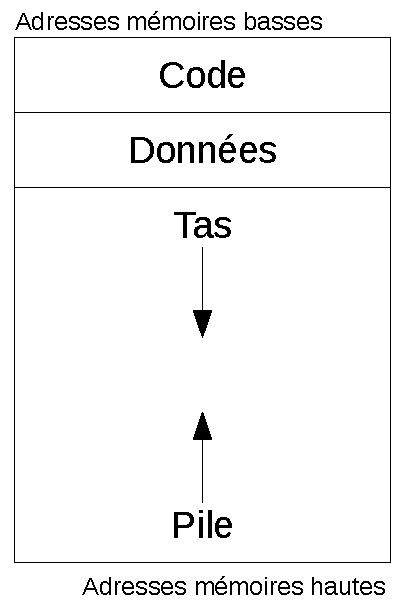
\includegraphics{supports/architecture/pile.pdf}
% % PSTricks TeX macro
% Title: /home/aurelien/RapportsLatex/these/supports/architecture/pile2.dia
% Creator: Dia v0.97.2
% CreationDate: Mon Jun 30 11:09:51 2014
% For: aurelien
% \usepackage{pstricks}
% The following commands are not supported in PSTricks at present
% We define them conditionally, so when they are implemented,
% this pstricks file will use them.
\ifx\setlinejoinmode\undefined
  \newcommand{\setlinejoinmode}[1]{}
\fi
\ifx\setlinecaps\undefined
  \newcommand{\setlinecaps}[1]{}
\fi
% This way define your own fonts mapping (for example with ifthen)
\ifx\setfont\undefined
  \newcommand{\setfont}[2]{}
\fi
\pspicture(-360.050000,-21.152500)(-349.950000,-3.386313)
\psscalebox{1.000000 -1.000000}{
\newrgbcolor{dialinecolor}{0.000000 0.000000 0.000000}%
\psset{linecolor=dialinecolor}
\newrgbcolor{diafillcolor}{1.000000 1.000000 1.000000}%
\psset{fillcolor=diafillcolor}
\psset{linewidth=0.100000cm}
\psset{linestyle=solid}
\psset{linestyle=solid}
\setlinejoinmode{0}
\newrgbcolor{dialinecolor}{1.000000 1.000000 1.000000}%
\psset{linecolor=dialinecolor}
\pspolygon*(-360.000000,5.000000)(-360.000000,20.000000)(-350.000000,20.000000)(-350.000000,5.000000)
\newrgbcolor{dialinecolor}{0.000000 0.000000 0.000000}%
\psset{linecolor=dialinecolor}
\pspolygon(-360.000000,5.000000)(-360.000000,20.000000)(-350.000000,20.000000)(-350.000000,5.000000)
\setfont{Helvetica}{0.800000}
\newrgbcolor{dialinecolor}{0.000000 0.000000 0.000000}%
\psset{linecolor=dialinecolor}
\rput[l](-360.000000,4.000000){\psscalebox{1 -1}{addresses mémoire basses}}
\setfont{Helvetica}{0.800000}
\newrgbcolor{dialinecolor}{0.000000 0.000000 0.000000}%
\psset{linecolor=dialinecolor}
\rput[l](-359.000000,21.000000){\psscalebox{1 -1}{addresses mémoire hautes}}
\psset{linewidth=0.100000cm}
\psset{linestyle=solid}
\psset{linestyle=solid}
\setlinejoinmode{0}
\newrgbcolor{dialinecolor}{1.000000 1.000000 1.000000}%
\psset{linecolor=dialinecolor}
\pspolygon*(-360.000000,5.000000)(-360.000000,7.000000)(-350.000000,7.000000)(-350.000000,5.000000)
\newrgbcolor{dialinecolor}{0.000000 0.000000 0.000000}%
\psset{linecolor=dialinecolor}
\pspolygon(-360.000000,5.000000)(-360.000000,7.000000)(-350.000000,7.000000)(-350.000000,5.000000)
\setfont{Helvetica}{0.800000}
\newrgbcolor{dialinecolor}{0.000000 0.000000 0.000000}%
\psset{linecolor=dialinecolor}
\rput[l](-357.000000,6.000000){\psscalebox{1 -1}{}}
\setfont{Helvetica}{0.800000}
\newrgbcolor{dialinecolor}{0.000000 0.000000 0.000000}%
\psset{linecolor=dialinecolor}
\rput(-355.000000,6.000000){\psscalebox{1 -1}{Code}}
\psset{linewidth=0.100000cm}
\psset{linestyle=solid}
\psset{linestyle=solid}
\setlinejoinmode{0}
\newrgbcolor{dialinecolor}{1.000000 1.000000 1.000000}%
\psset{linecolor=dialinecolor}
\pspolygon*(-360.000000,7.000000)(-360.000000,9.000000)(-350.000000,9.000000)(-350.000000,7.000000)
\newrgbcolor{dialinecolor}{0.000000 0.000000 0.000000}%
\psset{linecolor=dialinecolor}
\pspolygon(-360.000000,7.000000)(-360.000000,9.000000)(-350.000000,9.000000)(-350.000000,7.000000)
\setfont{Helvetica}{0.800000}
\newrgbcolor{dialinecolor}{0.000000 0.000000 0.000000}%
\psset{linecolor=dialinecolor}
\rput[l](-357.000000,8.000000){\psscalebox{1 -1}{}}
\setfont{Helvetica}{0.800000}
\newrgbcolor{dialinecolor}{0.000000 0.000000 0.000000}%
\psset{linecolor=dialinecolor}
\rput(-355.000000,8.000000){\psscalebox{1 -1}{Données}}
\setfont{Helvetica}{0.800000}
\newrgbcolor{dialinecolor}{0.000000 0.000000 0.000000}%
\psset{linecolor=dialinecolor}
\rput(-355.000000,19.221250){\psscalebox{1 -1}{Pile}}
\newrgbcolor{dialinecolor}{1.000000 1.000000 1.000000}%
\psset{linecolor=dialinecolor}
\pspolygon*(-355.505000,9.405000)(-355.505000,10.152500)(-354.495000,10.152500)(-354.495000,9.405000)
\setfont{Helvetica}{0.800000}
\newrgbcolor{dialinecolor}{0.000000 0.000000 0.000000}%
\psset{linecolor=dialinecolor}
\rput(-355.000000,10.000000){\psscalebox{1 -1}{Tas}}
\psset{linewidth=0.100000cm}
\psset{linestyle=dotted,dotsep=0.200000}
\psset{linestyle=dotted,dotsep=0.200000}
\setlinecaps{0}
\newrgbcolor{dialinecolor}{0.000000 0.000000 0.000000}%
\psset{linecolor=dialinecolor}
\psline(-355.000000,11.000000)(-355.000000,12.513197)
\psset{linestyle=solid}
\setlinejoinmode{0}
\setlinecaps{0}
\newrgbcolor{dialinecolor}{0.000000 0.000000 0.000000}%
\psset{linecolor=dialinecolor}
\pspolygon*(-355.000000,12.888197)(-355.250000,12.388197)(-355.000000,12.513197)(-354.750000,12.388197)
\newrgbcolor{dialinecolor}{0.000000 0.000000 0.000000}%
\psset{linecolor=dialinecolor}
\pspolygon(-355.000000,12.888197)(-355.250000,12.388197)(-355.000000,12.513197)(-354.750000,12.388197)
\psset{linewidth=0.100000cm}
\psset{linestyle=dotted,dotsep=0.200000}
\psset{linestyle=dotted,dotsep=0.200000}
\setlinecaps{0}
\newrgbcolor{dialinecolor}{0.000000 0.000000 0.000000}%
\psset{linecolor=dialinecolor}
\psline(-355.000000,18.000000)(-355.000000,16.486803)
\psset{linestyle=solid}
\setlinejoinmode{0}
\setlinecaps{0}
\newrgbcolor{dialinecolor}{0.000000 0.000000 0.000000}%
\psset{linecolor=dialinecolor}
\pspolygon*(-355.000000,16.111803)(-354.750000,16.611803)(-355.000000,16.486803)(-355.250000,16.611803)
\newrgbcolor{dialinecolor}{0.000000 0.000000 0.000000}%
\psset{linecolor=dialinecolor}
\pspolygon(-355.000000,16.111803)(-354.750000,16.611803)(-355.000000,16.486803)(-355.250000,16.611803)
}\endpspicture
\missingfigure{!}
\caption{Organisation de la mémoire d'un processus}
\label{fig:mem_process}
\end{center}
\end{figure}

\begin{figure}
\begin{center}
% Graphic for TeX using PGF
% Title: /home/aurelien/these/supports/architecture/arch.dia
% Creator: Dia v0.97.2
% CreationDate: Wed Jun 18 11:06:57 2014
% For: aurelien
% \usepackage{tikz}
% The following commands are not supported in PSTricks at present
% We define them conditionally, so when they are implemented,
% this pgf file will use them.
\ifx\du\undefined
  \newlength{\du}
\fi
\setlength{\du}{15\unitlength}
\begin{tikzpicture}
\pgftransformxscale{1.000000}
\pgftransformyscale{-1.000000}
\definecolor{dialinecolor}{rgb}{0.000000, 0.000000, 0.000000}
\pgfsetstrokecolor{dialinecolor}
\definecolor{dialinecolor}{rgb}{1.000000, 1.000000, 1.000000}
\pgfsetfillcolor{dialinecolor}
\definecolor{dialinecolor}{rgb}{1.000000, 1.000000, 1.000000}
\pgfsetfillcolor{dialinecolor}
\fill (16.000000\du,5.800000\du)--(16.000000\du,14.300000\du)--(39.000000\du,14.300000\du)--(39.000000\du,5.800000\du)--cycle;
\pgfsetlinewidth{0.100000\du}
\pgfsetdash{}{0pt}
\pgfsetdash{}{0pt}
\pgfsetmiterjoin
\definecolor{dialinecolor}{rgb}{0.000000, 0.000000, 0.000000}
\pgfsetstrokecolor{dialinecolor}
\draw (16.000000\du,5.800000\du)--(16.000000\du,14.300000\du)--(39.000000\du,14.300000\du)--(39.000000\du,5.800000\du)--cycle;
% setfont left to latex
\definecolor{dialinecolor}{rgb}{0.000000, 0.000000, 0.000000}
\pgfsetstrokecolor{dialinecolor}
\node[anchor=west] at (16.450000\du,10.245000\du){};
% setfont left to latex
\definecolor{dialinecolor}{rgb}{0.000000, 0.000000, 0.000000}
\pgfsetstrokecolor{dialinecolor}
\node[anchor=west] at (22.000000\du,7.000000\du){Processeur};
\definecolor{dialinecolor}{rgb}{1.000000, 1.000000, 1.000000}
\pgfsetfillcolor{dialinecolor}
\fill (17.000000\du,8.000000\du)--(17.000000\du,10.000000\du)--(25.000000\du,10.000000\du)--(25.000000\du,8.000000\du)--cycle;
\pgfsetlinewidth{0.100000\du}
\pgfsetdash{}{0pt}
\pgfsetdash{}{0pt}
\pgfsetmiterjoin
\definecolor{dialinecolor}{rgb}{0.000000, 0.000000, 0.000000}
\pgfsetstrokecolor{dialinecolor}
\draw (17.000000\du,8.000000\du)--(17.000000\du,10.000000\du)--(25.000000\du,10.000000\du)--(25.000000\du,8.000000\du)--cycle;
% setfont left to latex
\definecolor{dialinecolor}{rgb}{0.000000, 0.000000, 0.000000}
\pgfsetstrokecolor{dialinecolor}
\node at (21.000000\du,9.206667\du){Unité de contrôle};
\definecolor{dialinecolor}{rgb}{1.000000, 1.000000, 1.000000}
\pgfsetfillcolor{dialinecolor}
\fill (27.000000\du,11.000000\du)--(27.000000\du,13.000000\du)--(38.102500\du,13.000000\du)--(38.102500\du,11.000000\du)--cycle;
\pgfsetlinewidth{0.100000\du}
\pgfsetdash{}{0pt}
\pgfsetdash{}{0pt}
\pgfsetmiterjoin
\definecolor{dialinecolor}{rgb}{0.000000, 0.000000, 0.000000}
\pgfsetstrokecolor{dialinecolor}
\draw (27.000000\du,11.000000\du)--(27.000000\du,13.000000\du)--(38.102500\du,13.000000\du)--(38.102500\du,11.000000\du)--cycle;
% setfont left to latex
\definecolor{dialinecolor}{rgb}{0.000000, 0.000000, 0.000000}
\pgfsetstrokecolor{dialinecolor}
\node at (32.551250\du,12.206667\du){Unité arithmétique et logique};
\definecolor{dialinecolor}{rgb}{1.000000, 1.000000, 1.000000}
\pgfsetfillcolor{dialinecolor}
\fill (28.000000\du,8.000000\du)--(28.000000\du,10.000000\du)--(32.225000\du,10.000000\du)--(32.225000\du,8.000000\du)--cycle;
\pgfsetlinewidth{0.100000\du}
\pgfsetdash{}{0pt}
\pgfsetdash{}{0pt}
\pgfsetmiterjoin
\definecolor{dialinecolor}{rgb}{0.000000, 0.000000, 0.000000}
\pgfsetstrokecolor{dialinecolor}
\draw (28.000000\du,8.000000\du)--(28.000000\du,10.000000\du)--(32.225000\du,10.000000\du)--(32.225000\du,8.000000\du)--cycle;
% setfont left to latex
\definecolor{dialinecolor}{rgb}{0.000000, 0.000000, 0.000000}
\pgfsetstrokecolor{dialinecolor}
\node at (30.112500\du,9.206667\du){Registres};
\pgfsetlinewidth{0.100000\du}
\pgfsetdash{}{0pt}
\pgfsetdash{}{0pt}
\pgfsetbuttcap
{
\definecolor{dialinecolor}{rgb}{0.000000, 0.000000, 0.000000}
\pgfsetfillcolor{dialinecolor}
% was here!!!
\pgfsetarrowsend{stealth}
\definecolor{dialinecolor}{rgb}{0.000000, 0.000000, 0.000000}
\pgfsetstrokecolor{dialinecolor}
\pgfpathmoveto{\pgfpoint{28.000033\du}{8.000024\du}}
\pgfpatharc{306}{235}{2.561783\du and 2.561783\du}
\pgfusepath{stroke}
}
\pgfsetlinewidth{0.100000\du}
\pgfsetdash{}{0pt}
\pgfsetdash{}{0pt}
\pgfsetbuttcap
{
\definecolor{dialinecolor}{rgb}{0.000000, 0.000000, 0.000000}
\pgfsetfillcolor{dialinecolor}
% was here!!!
\pgfsetarrowsend{stealth}
\definecolor{dialinecolor}{rgb}{0.000000, 0.000000, 0.000000}
\pgfsetstrokecolor{dialinecolor}
\pgfpathmoveto{\pgfpoint{27.000016\du}{11.000026\du}}
\pgfpatharc{329}{285}{3.342444\du and 3.342444\du}
\pgfusepath{stroke}
}
\pgfsetlinewidth{0.100000\du}
\pgfsetdash{}{0pt}
\pgfsetdash{}{0pt}
\pgfsetbuttcap
{
\definecolor{dialinecolor}{rgb}{0.000000, 0.000000, 0.000000}
\pgfsetfillcolor{dialinecolor}
% was here!!!
\pgfsetarrowsend{stealth}
\definecolor{dialinecolor}{rgb}{0.000000, 0.000000, 0.000000}
\pgfsetstrokecolor{dialinecolor}
\pgfpathmoveto{\pgfpoint{24.999562\du}{9.999435\du}}
\pgfpatharc{143}{128}{11.225061\du and 11.225061\du}
\pgfusepath{stroke}
}
\definecolor{dialinecolor}{rgb}{1.000000, 1.000000, 1.000000}
\pgfsetfillcolor{dialinecolor}
\fill (18.000000\du,2.503333\du)--(18.000000\du,4.450000\du)--(22.045000\du,4.450000\du)--(22.045000\du,2.503333\du)--cycle;
\pgfsetlinewidth{0.100000\du}
\pgfsetdash{}{0pt}
\pgfsetdash{}{0pt}
\pgfsetmiterjoin
\definecolor{dialinecolor}{rgb}{0.000000, 0.000000, 0.000000}
\pgfsetstrokecolor{dialinecolor}
\draw (18.000000\du,2.503333\du)--(18.000000\du,4.450000\du)--(22.045000\du,4.450000\du)--(22.045000\du,2.503333\du)--cycle;
% setfont left to latex
\definecolor{dialinecolor}{rgb}{0.000000, 0.000000, 0.000000}
\pgfsetstrokecolor{dialinecolor}
\node at (20.022500\du,3.683333\du){Mémoire};
\definecolor{dialinecolor}{rgb}{1.000000, 1.000000, 1.000000}
\pgfsetfillcolor{dialinecolor}
\fill (18.000000\du,16.000000\du)--(18.000000\du,18.000000\du)--(22.000000\du,18.000000\du)--(22.000000\du,16.000000\du)--cycle;
\pgfsetlinewidth{0.100000\du}
\pgfsetdash{}{0pt}
\pgfsetdash{}{0pt}
\pgfsetmiterjoin
\definecolor{dialinecolor}{rgb}{0.000000, 0.000000, 0.000000}
\pgfsetstrokecolor{dialinecolor}
\draw (18.000000\du,16.000000\du)--(18.000000\du,18.000000\du)--(22.000000\du,18.000000\du)--(22.000000\du,16.000000\du)--cycle;
% setfont left to latex
\definecolor{dialinecolor}{rgb}{0.000000, 0.000000, 0.000000}
\pgfsetstrokecolor{dialinecolor}
\node at (20.000000\du,17.206667\du){Entrées};
\definecolor{dialinecolor}{rgb}{1.000000, 1.000000, 1.000000}
\pgfsetfillcolor{dialinecolor}
\fill (24.000000\du,16.000000\du)--(24.000000\du,18.000000\du)--(28.000000\du,18.000000\du)--(28.000000\du,16.000000\du)--cycle;
\pgfsetlinewidth{0.100000\du}
\pgfsetdash{}{0pt}
\pgfsetdash{}{0pt}
\pgfsetmiterjoin
\definecolor{dialinecolor}{rgb}{0.000000, 0.000000, 0.000000}
\pgfsetstrokecolor{dialinecolor}
\draw (24.000000\du,16.000000\du)--(24.000000\du,18.000000\du)--(28.000000\du,18.000000\du)--(28.000000\du,16.000000\du)--cycle;
% setfont left to latex
\definecolor{dialinecolor}{rgb}{0.000000, 0.000000, 0.000000}
\pgfsetstrokecolor{dialinecolor}
\node at (26.000000\du,17.206667\du){Sorties};
\pgfsetlinewidth{0.100000\du}
\pgfsetdash{}{0pt}
\pgfsetdash{}{0pt}
\pgfsetbuttcap
{
\definecolor{dialinecolor}{rgb}{0.000000, 0.000000, 0.000000}
\pgfsetfillcolor{dialinecolor}
% was here!!!
\pgfsetarrowsend{stealth}
\definecolor{dialinecolor}{rgb}{0.000000, 0.000000, 0.000000}
\pgfsetstrokecolor{dialinecolor}
\pgfpathmoveto{\pgfpoint{19.011333\du}{4.449795\du}}
\pgfpatharc{202}{159}{4.783839\du and 4.783839\du}
\pgfusepath{stroke}
}
\pgfsetlinewidth{0.100000\du}
\pgfsetdash{}{0pt}
\pgfsetdash{}{0pt}
\pgfsetbuttcap
{
\definecolor{dialinecolor}{rgb}{0.000000, 0.000000, 0.000000}
\pgfsetfillcolor{dialinecolor}
% was here!!!
\pgfsetarrowsend{stealth}
\definecolor{dialinecolor}{rgb}{0.000000, 0.000000, 0.000000}
\pgfsetstrokecolor{dialinecolor}
\pgfpathmoveto{\pgfpoint{20.999967\du}{8.000604\du}}
\pgfpatharc{4}{-33}{5.798338\du and 5.798338\du}
\pgfusepath{stroke}
}
\pgfsetlinewidth{0.100000\du}
\pgfsetdash{}{0pt}
\pgfsetdash{}{0pt}
\pgfsetbuttcap
{
\definecolor{dialinecolor}{rgb}{0.000000, 0.000000, 0.000000}
\pgfsetfillcolor{dialinecolor}
% was here!!!
\pgfsetarrowsend{stealth}
\definecolor{dialinecolor}{rgb}{0.000000, 0.000000, 0.000000}
\pgfsetstrokecolor{dialinecolor}
\pgfpathmoveto{\pgfpoint{19.000096\du}{9.999695\du}}
\pgfpatharc{198}{144}{6.720258\du and 6.720258\du}
\pgfusepath{stroke}
}
\pgfsetlinewidth{0.100000\du}
\pgfsetdash{}{0pt}
\pgfsetdash{}{0pt}
\pgfsetbuttcap
{
\definecolor{dialinecolor}{rgb}{0.000000, 0.000000, 0.000000}
\pgfsetfillcolor{dialinecolor}
% was here!!!
\pgfsetarrowsend{stealth}
\definecolor{dialinecolor}{rgb}{0.000000, 0.000000, 0.000000}
\pgfsetstrokecolor{dialinecolor}
\pgfpathmoveto{\pgfpoint{26.000003\du}{16.000021\du}}
\pgfpatharc{353}{315}{10.161156\du and 10.161156\du}
\pgfusepath{stroke}
}
\pgfsetlinewidth{0.100000\du}
\pgfsetdash{}{0pt}
\pgfsetdash{}{0pt}
\pgfsetbuttcap
{
\definecolor{dialinecolor}{rgb}{0.000000, 0.000000, 0.000000}
\pgfsetfillcolor{dialinecolor}
% was here!!!
\pgfsetarrowsend{stealth}
\definecolor{dialinecolor}{rgb}{0.000000, 0.000000, 0.000000}
\pgfsetstrokecolor{dialinecolor}
\pgfpathmoveto{\pgfpoint{24.999678\du}{8.199859\du}}
\pgfpatharc{114}{78}{4.877392\du and 4.877392\du}
\pgfusepath{stroke}
}
\pgfsetlinewidth{0.100000\du}
\pgfsetdash{}{0pt}
\pgfsetdash{}{0pt}
\pgfsetbuttcap
{
\definecolor{dialinecolor}{rgb}{0.000000, 0.000000, 0.000000}
\pgfsetfillcolor{dialinecolor}
% was here!!!
\pgfsetarrowsend{stealth}
\definecolor{dialinecolor}{rgb}{0.000000, 0.000000, 0.000000}
\pgfsetstrokecolor{dialinecolor}
\pgfpathmoveto{\pgfpoint{33.300602\du}{10.953459\du}}
\pgfpatharc{18}{-64}{2.044555\du and 2.044555\du}
\pgfusepath{stroke}
}
\end{tikzpicture}

\caption{Architecture de Harvard modifiée}
\label{fig:arch_harvard_mod}
\end{center}
\end{figure}

\paragraph{Jeu d'instructions.}
\todo{notation intel?}
Les processeurs Intel \xq\ utilisent un jeu d'instruction complexe (CISC). La représentation d'une instruction en une suite d'octets inclut principalement un type opération (opcode\todo{opcode?}) et ses arguments. Des informations supplémentaire peuvent être codées dans l'instruction, comme des préfixes. Le format des instructions détaillé est donné figure \ref{fig:format_insts_x86}.
L'instruction \texttt{mov ecx, 0x080490a4} de la figure \ref{fig:text_helloworld}, codée sur \texttt{b9 a4 90 04 08} est composée de l'opcode \texttt{b8+r} indiquant une opération de copie d'une valeur immédiate vers un registre. Ici le modificateur r est égal à 1, ce qui indique que le registre concerné est ecx. La valeur à copier vers le registre est 0x080490a4 soient les octets \texttt{a4 90 04 08} codés en petit-boutistes \todo{endianness ??}, c'est à dire que les mots de poids faibles sont écrits en premiers, à l'inverse de l'écriture usuelle.
Il s'agit d'une assignation immédiate et la valeur à copier vers \texttt{ecx} est la valeur immédiate.
Le décalage permet de modifier une instruction d'adressage indirect comme \texttt{mov ecx, [eax]}, écrivant le contenu en mémoire à l'adresse \texttt{eax} dans le registre \texttt{ecx} en \texttt{mov ebx, [eax+d]} où \texttt{d} est le décalage.
Enfin les préfixes permettent par exemple de répéter plusieurs fois l'instruction jusqu'à ce qu'une condition sur un registre soit remplie.

\begin{figure}
\begin{center} 
\begin{tabular}{|c|c|c|c|c|c|}
\hline
% Prefixe & Opcode & Modificateur & SIB & Déplacement d'octet & Adressage\\
% 1 à 4 & 1 à 3 & 0 ou 1 & 0 ou 1 & 0 à 4 & 0 à 4\\
Prefixe & Opcode & Modificateur & Décalage & Valeur immédiate\\
1 à 4 & 1 à 3 & 0 à 2 & 0 à 4 & 0 à 4\\
\hline
\end{tabular}
\end{center} 
\caption{Format d'une instruction \xq}
\label{fig:format_insts_x86}
\end{figure}

\paragraph{Intuition de sémantique.}
% ~\\
% \todo[inline]{assignations (déplacement en mémoire)\\
% opérations arithmétique\\
% controle de flot inconditionnel\\
% conditionnel}
% 
% \todo[inline]{effets de bords\\
% explicites\\
% implicites}

Bien que la documentation exhaustive d'Intel pour les processeurs \xq\ et \xs\ \cite{intel_vol2} détaille plusieurs centaines d'instructions, elles peuvent être regroupées en 3 classes.
Prenons l'instruction \texttt{mov}. Elle sert à copier des informations depuis une zone (mémoire ou registre) vers une autre zone.
Ainsi \texttt{mov eax, [ebx+10]} copie la valeur à l'adresse \texttt{ebx+10} dans le registre \eax. 
Cette instruction est déclinée en plusieurs dizaines de variantes selon la taille et le type des opérandes copiés.

Une seconde catégorie d'instructions permet de gérer les opérations arithmétiques sur les octets en mémoire et dans les registres.
Une instructions comme \texttt{add eax, ebx} ajoute la valeur de \ebx\ à celle de \eax\ et stocke le résultat de l'opération dans \eax.
Ce type d'opération combine en fait une opération arithmétique et une assignation. 
On peut y inclure l'instruction \cmp\ qui compare deux valeurs et met à jour les registres de tests. 
Ces registres indiquent entre autres si le signe du résultat d'une opération ainsi que si elle a provoqué un débordement d'entier (dans le cas où le résultat est trop grand pour être stocké sur un entier).
En fait les instructions arithmétiques comme \add\ provoquent aussi une mise à jour de ces registres : il s'agit d'une assignation implicite.

Les instructions précédemment décrites sont séquentielles et ne modifient pas l'ordre d'exécution d'une instruction. 
Après l'exécution d'une instruction de type \mov\ à l'adresse $a$ codée sur $n$ octets, l'instruction située à l'adresse $a+n$.
Le dernier type d'instruction modifie le flot de contrôle du programme et effectuent des sauts à des adresses spécifiées dans le programme.
Ces sauts peuvent être inconditionnels comme un \texttt{jmp 8048085} qui provoque un saut à l'adresse \texttt{8048085} ou le saut dynamique \texttt{jmp eax} dont l'adresse cible du saut est la valeur de \eax.
Les sauts peuvent aussi être conditionnels : \texttt{je +10}, à l'adresse $a$ et de taille $n$, sera suivie de l'instruction à l'adresse $a+10$ si le registre ZF vaut 1 (en cas d'égalité) et de l'instruction à l'adresse $a+n$ dans le cas contraire.


\section{Désassemblage}
Le désassemblage est l'opération inverse de l'assemblage : il consiste à récupérer le code assembleur source du binaire.
Cette tâche semble particulièrement simple puisque l'assemblage consiste simplement à trouver les octets correspondants à chaque instruction à l'aide de la documentation officielle du processeur puis à mettre en forme le fichier binaire en remplissant correctement ses entêtes et ses sections.
Pourtant on a vu que, dans le modèle d'Harvard modifié, les données et le code peuvent être mêlés. 
En particulier les parties de données (comme la section .data) peuvent être exécutées. 
De même les sections de code peuvent contenir des informations destinées à être simplement lues ou modifiées mais jamais exécutées.
La difficulté du désassemblage consiste donc à séparer les parties potentiellement exécutables des données.

Ainsi un désassemblage à priori cohérent de \helloworld\ consisterait à considérer les deux sections comme contenant du code potentiellement exécutable. Ce désassemblage sera composé de la section .text déjà désassemblé Figure \ref{fig:text_helloworld} et la section .data donnée Figure \ref{fig:data_exec_helloworld}.
Ce désassemblage n'est pas correct et on peut le prédire. 
On connaît le point d'entrée du binaire, qui est l'adresse \texttt{8048080} dans la section .text.
Les instructions exécutées dans la section .text à la suite du point d'entrée sont séquentielles et ne peuvent détourner l'exécution vers la section .data. 
Le code désassemblé dans cette section n'est donc pas atteignable. Dans ce cas on sait alors que la section .data ne contient pas de code et ne doit pas être désassemblée.

\paragraph{Utilisation de sauts dynamiques.}
En pratique un programme est constitué d'un grand nombre d'instructions de saut et notamment de sauts dynamiques de type \texttt{jmp eax}.
Ce type d'instructions posent un souci lors de l'analyse : sans connaître précisément la ou les valeurs potentielles d'\eax, impossible de prédire la cible du saut et donc de savoir le code potentiellement exécuté à la suite de cette instruction.
Dans l'exemple du \helloworld, si une telle instruction est présente dans la section .text, il devient difficile d'exclure l'exécution possible de code dans la section .data.

\paragraph{Difficulté théorique du désassemblage.}
On a vu que le problème du désassemblage tient dans la difficulté de séparer les parties de code potentiel des parties de données.
Plus précisément le but du désassemblage d'un programme P est alors de déterminer l'ensemble des adresses $a$ du programme pour lesquelles il existe une entrée I telle que l'exécution de P(I) atteint $a$.
Nous citons ici un argument tiré de la thèse de Joan Calvet \cite{Calvet2013} montrant le caractère indécidable de ce problème en réduisant le problème de l'arrêt à celui-ci.

Supposons que le problème soit décidable et notons, pour tout programme P, $CODE(P)$ l'ensemble des adresses des instructions de P atteignables lors de l'exécution de P. Pour tout programme P et toute entrée I à P, on peut définir le programme P' suivant qui ne prend pas d'entrée :

\begin{center}
\begin{tabular}{|l|l|}
\hline
Adresse & Commande \\
\hline
0 & call P(I)\\
$\alpha$ & halt \\
\hline
\end{tabular}
\end{center}

Deux cas sont alors possibles.
\begin{itemize}
 \item Soit $\alpha\in\ CODE(P')$ et dans ce cas l'exécution atteint l'adresse $\alpha$ donc le programme P termine sur l'entrée I.
 \item Soit $\alpha\notin\ CODE(P')$ donc le programme P ne termine pas sur l'entrée I.
\end{itemize}
~\\
On en déduit donc que le désassemblage permet de résoudre le problème de l'arrêt qui est pourtant connu pour être indécidable ; c'est absurde.
Ainsi le problème du désassemblage est indécidable.


\begin{figure}
\begin{center}
\begin{tabular}{|c|c|l|l|}
\hline
Emplacement dans le fichier & Adresses de chargement & Octets & Instruction\\ 
\hline
94 & 80490a4 & 48    & dec    eax			\\
95 & 80490a5 & 65    & gs				\\
96 & 80490a6 & 6c    & ins    BYTE PTR es:[edi],dx	\\
97 & 80490a7 & 6c    & ins    BYTE PTR es:[edi],dx	\\
98 & 80490a8 & 6f    & outs   dx,DWORD PTR ds:[esi]	\\
99 & 80490a9 & 2c 20 & sub    al,0x20			\\
9b & 80490ab & 77 6f & ja     0x804911c			\\
9d & 80490ad & 72 6c & jb     0x804911b			\\
9f & 80490af & 64    & fs				\\
a0 & 80490b0 & 0a    & .byte 0xa			\\
\hline
\end{tabular}
\end{center}
\caption{Section .data de \helloworld\ désassemblée comme du code}
\label{fig:data_exec_helloworld}
\end{figure}

\todo[inline]{Analyse statique, analyse dynamique ?\\
linear sweep, recursive traversal, speculative disassembly}

\subsection{Analyse statique}
\paragraph{Linear sweep.}
\paragraph{Recursive disassembly.}

\subsection{Analyse dynamique}

% \paragraph{Décompilation.}

\section{Obfuscations}
\subsection{Auto-modification}
\todo[inline]{
Qu'est-ce ? \\
Autorisé par l'OS (NX ?) \\
Comment ? \\
Exemple
}

\subsection{Obscurcissement statique}
\todo[inline]{
Ajout de junk code \\
Détournement de calls \\
Chevauchements \\
Prédicats opaques\\
}
\todo[inline]{
Réorganisation du code \\
Aplatissement de CFG \\
}

% \section{Difficulté calculatoire de l'analyse de binaire}
% \subsection{Désassemblage}
% \subsection{Décompilation}

\DontFrameThisInToc
\chapter{Désassemblage et analyse statique}
\todo[inline]{Sémantique, Layers\\ sémantique SM: SM-VSA + emulation BAP}
% Ici on parle d'assembleur

\section{Premiere section}
Ahah

\DontFrameThisInToc
\chapter{Analyse dynamique et hybride}
\todo[inline]{Limites analyse statique, analyse dynamique et waves\\ disasm.py}
% Ici on parle d'assembleur

\section{Premiere section}
Ahah

\DontFrameThisInToc
\chapter{Résultats}
% Ici on parle d'assembleur

\section{Premiere section}
Ahah

% \WriteThisInToc
% \FrameThisInToc
% \NumberThisInToc
\part{Analyse morphologique}
\DontFrameThisInToc
\chapter{Analyse de graphes et algorithmes}

\DontFrameThisInToc
\chapter{Validation de l'approche}
\todo[inline]{Perfs + FP/FN}

\DontFrameThisInToc
\chapter{Application à la détection de librairies}
\todo[inline]{Cas Waledac / OpenSSL}

\DontFrameThisInToc
\chapter{Cas d'étude : Duqu et Stuxnet}

\PutLineInToc
% \PutNewPageInToc

%-------------------------------------------------------------------
%              L'index (toujours sur deux colonnes)
%-------------------------------------------------------------------
\BeginIndWith{Voici un index}
\PrintIndex

\onecolumn

%-------------------------------------------------------------------
%                       La bibliographie
%-------------------------------------------------------------------

% La bibliographie (comme d'habitude)

\nocite{*}
% \bibliographystyle{unsrt}
% \bibliographystyle{named}
% \bibliography{these}
\printbibliography

\NumberAbstractPages
\begin{ThesisAbstract}
  \begin{FrenchAbstract}
    Résumé.
    \KeyWords{a, b, c.}
  \end{FrenchAbstract}
  \begin{EnglishAbstract}
    Abstract.
    \KeyWords{a, b, c.}
  \end{EnglishAbstract}
\end{ThesisAbstract}


\end{document}


